% ============================================================================
% Evidence-Bounded CAD Repair for Simulation Meshing
% Hexera CAD Repair System - technical paper (mid-length: brief enough to read,
% full enough to argue from). The 15-page long form is full-paper.tex.
%
% Overleaf: upload this file, compiler pdfLaTeX, main document main.tex,
% recompile twice. Self-contained: TikZ figures, no external images.
% Locally: latexmk -pdf main.tex
%
% Every number comes from a committed evidence README under
% devtools/validation/evidence/ or a spec under docs/superpowers/specs/.
% Update the paper with the evidence, never ahead of it.
%
% HOUSE STYLE (keep it consistent, this is what makes it read as one document):
%   - Block paragraphs: no first-line indent, one blank line of space between.
%     Do not mix in \indent or \noindent; the preamble handles it.
%   - Run-in lead-ins are \topic{...}, never a bare \textbf at the start of a
%     paragraph: \topic keeps the spacing and the period consistent.
%   - Lists hang from the text block with label alignment left; set only with
%     the \setlist defaults below, never per-list.
% ============================================================================
\documentclass[10pt,onecolumn]{article}

\usepackage[T1]{fontenc}
\usepackage{charter}
\usepackage[scaled=0.84]{beramono}
\usepackage[letterpaper,margin=0.95in]{geometry}
\usepackage{microtype}
\setlength{\emergencystretch}{1.2em}
\usepackage{booktabs}
\usepackage{tabularx}
\usepackage{array}
\usepackage{amsmath,amssymb}
\usepackage{algorithm}
\usepackage{algpseudocode}
\usepackage{float}
\usepackage{tikz}
\usetikzlibrary{arrows.meta,positioning,calc}
\usepackage[labelfont=bf,font=small,skip=5pt]{caption}
\usepackage{enumitem}
\usepackage{titlesec}
\usepackage{fancyhdr}
\usepackage{seqsplit}
\usepackage{multicol}
\usepackage[hidelinks]{hyperref}

% ---- paragraph style: block, not indented, applied everywhere -------------
\setlength{\parindent}{0pt}
\setlength{\parskip}{0.62\baselineskip}
\setlength{\abovedisplayskip}{6pt}
\setlength{\belowdisplayskip}{6pt}

% ---- headings --------------------------------------------------------------
\titleformat{\section}{\normalfont\large\bfseries}{\thesection}{0.7em}{}
\titleformat{\subsection}{\normalfont\normalsize\bfseries}{\thesubsection}{0.7em}{}
\titlespacing*{\section}{0pt}{1.15\baselineskip}{0.35\baselineskip}
\titlespacing*{\subsection}{0pt}{0.85\baselineskip}{0.25\baselineskip}
%: run-in lead-in for a paragraph. One command, so every lead-in looks alike.
\newcommand{\topic}[1]{\textbf{#1.}\hspace{0.5em}\ignorespaces}

% ---- lists: hang from the text block, even spacing -------------------------
\setlist{nosep}
%: labelindent + labelwidth + labelsep == leftmargin, so a wrapped line lands
%: under the first word of its item rather than back at the margin.
\setlist[itemize]{leftmargin=1.5em,labelindent=0pt,labelwidth=0.8em,labelsep=0.7em,
                  align=left,label=\textbullet,itemsep=5pt,topsep=5pt}
\setlist[enumerate]{leftmargin=2.1em,labelindent=0pt,labelwidth=1.4em,labelsep=0.7em,
                    align=left,label=\arabic*.,itemsep=5pt,topsep=5pt}

\pagestyle{fancy}
\fancyhf{}
\renewcommand{\headrulewidth}{0.4pt}
\fancyhead[C]{\footnotesize\itshape Hexera CAD Repair System --- Technical Paper}
\fancyfoot[C]{\thepage}
\fancypagestyle{plain}{\fancyhf{}\renewcommand{\headrulewidth}{0pt}\fancyfoot[C]{\thepage}}

\newcommand{\code}[1]{\texttt{\small #1}}
\newcommand{\lcode}[1]{\texttt{\small\seqsplit{#1}}}
\newcommand{\tablecode}{\renewcommand{\code}[1]{{\fontsize{7.2}{8.6}\selectfont\ttfamily ##1}}}
\newcolumntype{L}[1]{>{\raggedright\arraybackslash}p{#1}}

\tikzset{
  blk/.style={draw,thin,rectangle,align=center,inner sep=2.5pt,font=\scriptsize,
              minimum height=8mm,text width=20mm},
  sblk/.style={blk,text width=16mm,minimum height=5.5mm},
  dblk/.style={blk,dashed},
  ar/.style={-{Latex[length=1.5mm,width=1.1mm]},thin},
  lbl/.style={font=\scriptsize\itshape,text=black!60},
}

\title{\vspace{-1.3cm}\bfseries Evidence-Bounded CAD Repair for Simulation Meshing\\[0.2em]
       \large\normalfont\itshape The Hexera CAD Repair System: design, guarantees and measured results}
\author{Hexera Engineering}
\date{Technical Paper --- November 2026}

\begin{document}
\maketitle
\thispagestyle{plain}

% =============================================================== 1 ==========
\section{Overview}

\topic{The problem} Imported CAD breaks meshing before a solver ever runs. Parts arrive from many
CAD systems through a neutral format, usually STEP, and that round trip is lossy. Faces lose the
edges they shared, so closed shells open up. Trimming curves drift from the surfaces they bound.
Slivers and nanometre-long edges appear throughout. Some of it violates the validity rules of the boundary
representation (B-rep); the rest is valid and still unmeshable. Either way the mesh generator
refuses the part, and an analyst repairs it by hand, which must be repeated for every revision of
the part.

\topic{What CRS does} The Hexera CAD Repair System sits between CAD intake and mesh generation. It
locates each defect, applies one narrow kernel operation to a snapshot, measures the result
independently, and keeps the edit only when that measurement shows progress inside limits taken
from the original upload. The upload itself is never modified, and a rejected candidate never
becomes output.

\topic{Why verification is the hard part} Healing toolkits are widely available, and the usual
pattern is to run one and accept its result. That is weaker than it looks. A healing call reports
success once it has run out of errors to report, which it can reach by inflating tolerances until
the kernel stops checking them, or by removing the small features that drew the complaint. The
second route is defeaturing, and a defeatured model answers a different physics question than the
one it was built for. Neither route leaves a record a reviewer can audit. CRS therefore does
not accept a kernel's success flag as evidence. Every edit is a transaction, judged after the fact
against four conditions.

\begin{enumerate}
  \item \topic{Kernel floor} Valid shape, no solid lost, no undeclared face removed, meshable faces
        remain. No operation, directive or model package can waive this.
  \item \topic{Caps measured against the upload} Tolerance at most 0.1\,mm; surface movement at most
        0.001 of the part diagonal; area and volume within 2\% of the upload plus whatever the
        operation declared. Because the comparison is always against the \emph{upload} and never the
        previous step, a sequence of individually small edits cannot accumulate into a large one.
  \item \topic{Progress} Independent re-inspection shows the target defect gone or materially
        improved, with no new finding of warning severity or worse.
  \item \topic{Declaration honesty} An operation whose measured change exceeds what it declared is
        refused even when the change itself was harmless. The refusal is for misdescribing the
        edit, since every later check reads the declaration as the record of what happened.
\end{enumerate}

\topic{What it refuses to do} CRS does not infer design intent, does not defeature to satisfy a
mesher, and does not certify a simulation. Where the correct change depends on engineering
judgement, it routes the part to a person with the evidence attached. The bias towards refusal
follows from the cost of each kind of error: a wrongly rejected edit costs a missed repair, while a
wrongly accepted one delivers altered geometry to a customer. An unsupported defect ends in refusal, and so does
an ambiguous target, an exhausted budget, or a measurement that could not be taken.

\begin{figure}[h]
\centering
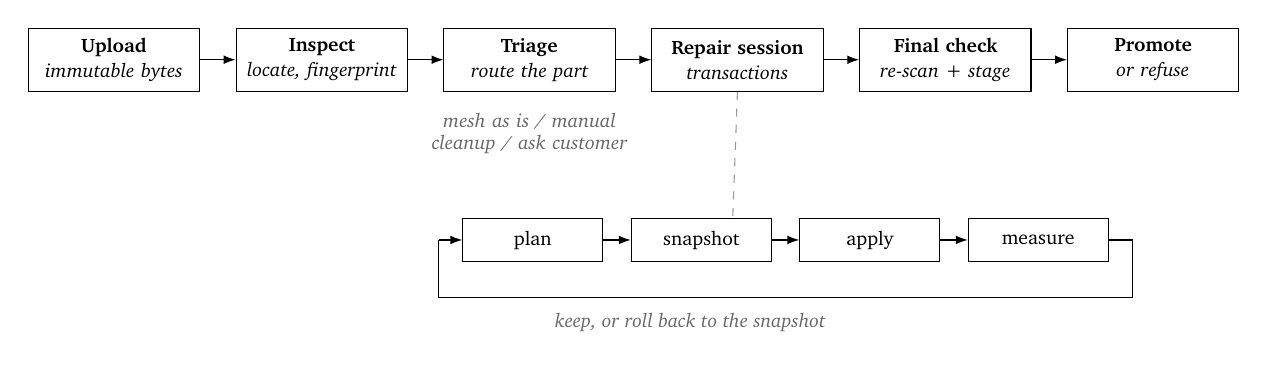
\begin{tikzpicture}[node distance=4.5mm]
  \node[blk] (up)  {\textbf{Upload}\\[1pt]\scriptsize\itshape immutable bytes};
  \node[blk,right=of up]  (ins) {\textbf{Inspect}\\[1pt]\scriptsize\itshape locate, fingerprint};
  \node[blk,right=of ins] (tri) {\textbf{Triage}\\[1pt]\scriptsize\itshape route the part};
  \node[blk,right=of tri] (ses) {\textbf{Repair session}\\[1pt]\scriptsize\itshape transactions};
  \node[blk,right=of ses] (fin) {\textbf{Final check}\\[1pt]\scriptsize\itshape re-scan + stage};
  \node[blk,right=of fin] (pro) {\textbf{Promote}\\[1pt]\scriptsize\itshape or refuse};
  \foreach \a/\b in {up/ins,ins/tri,tri/ses,ses/fin,fin/pro} \draw[ar] (\a) -- (\b);
  \node[lbl,below=1.5mm of tri,text width=26mm,align=center]
       {mesh as is / manual cleanup / ask customer};

  \node[sblk,below=16mm of ses,xshift=-26mm] (p1) {plan};
  \node[sblk,right=3.5mm of p1] (p2) {snapshot};
  \node[sblk,right=3.5mm of p2] (p3) {apply};
  \node[sblk,right=3.5mm of p3] (p4) {measure};
  \foreach \a/\b in {p1/p2,p2/p3,p3/p4} \draw[ar] (\a) -- (\b);
  \coordinate (ra) at ($(p4.east)+(3mm,0)$);
  \coordinate (rb) at ($(p1.west)+(-3mm,0)$);
  \coordinate (rlow) at ($(p1.south)+(0,-4.5mm)$);
  \draw[thin] (p4.east) -- (ra) -- (ra|-rlow) -- (rb|-rlow) -- (rb);
  \draw[ar] (rb) -- (p1.west);
  \node[lbl,below=0.8mm of rlow,xshift=20mm] {keep, or roll back to the snapshot};
  \draw[dashed,thin,black!40] (ses.south) -- ($(p2.north)+(4mm,0)$);
\end{tikzpicture}
\caption{The pipeline. Inside the session each operation is a transaction against a snapshot; a
candidate failing any of the four conditions is rolled back. Only a part that passes the final
re-inspection and stages for the chosen mesh engine is promoted, as a separate artefact.}
\label{fig:pipeline}
\end{figure}

\topic{What it delivers today} On the 331-file OCCT corpus the catalogue repairs 430 defects, and
every file promoted as a repaired artefact passes an independent final check. On a full Formula
1000 vehicle body it cleared the blocking invalidity, preserved all 8 solids, and halved the time
the mesh engine needed to stage the part. Region scoping then cut the proof cost of a run by about
a factor of ten with no change in outcomes and no change to clean parts.

Three extensions build on that core, and Section~\ref{sec:how} describes each: a
\emph{region-scoped driver}, so that a local edit needs only a local proof; a \emph{mesh probe},
which turns mesher failures into located defects; and a \emph{model author} paired with a separate
reviewer that sees measured evidence only. Section~\ref{sec:method} sets out the evaluation method
and Section~\ref{sec:results} the results, including the negative ones.

\topic{Where the system stands} Everything measured in this paper is the deterministic path: the
catalogue, the region driver, the probe and the caps. A second generation of the loop --- goal
profiles, a ladder of cheap in-loop oracles, a bounded investigator that may look, measure, probe
and edit on a throwaway copy, a tournament of candidate repairs rehearsed on clones, and a two-tier
reviewer --- is built, tested and merged, and is described in Section~\ref{sec:v3}. Its first
measurement is Section~\ref{sec:v3results}, where any value not yet measured is printed as
\textbf{[PENDING]} rather than as a number. Every one of its posture flags defaults off, and
Table~\ref{tab:v3status} states for each piece what is missing. Read Section~\ref{sec:v3} as
design and as code that exists. The only gains this paper reports for it are the ones
Section~\ref{sec:v3results} prints.

% =============================================================== 2 ==========
\section{Context}

\topic{Healing toolkits} OpenCASCADE's ShapeFix and ShapeUpgrade packages~\cite{occt}, and the
equivalents inside commercial pre-processors, supply the primitive operations CRS uses: sewing,
wire repair, small-edge and small-face removal, and splitting closed faces. They do not supply
independent verification, limits measured against the original, rollback, or an audit record. Those
are what CRS adds around them.

\topic{Meshing defective geometry directly} fTetWild~\cite{ftetwild} tetrahedralises
imperfect triangle soups inside a user-set envelope, and for many analyses that is the right tool.
It gives up the parametric B-rep, though, and our output must remain editable CAD that a customer
can re-open, inspect and re-mesh with any engine. CRS therefore repairs the CAD and changes no
mesher settings. Mesh quality in the element-shape sense~\cite{shewchuk,knupp} belongs to the
meshing stage and is out of scope here.

\topic{Models in refinement loops} Self-Refine~\cite{selfrefine} showed that a model can critique
and improve its own output across several tasks. Huang et al.~\cite{huang} established the limit:
without an external oracle, intrinsic self-correction often makes results \emph{worse}. A recent
study of agent loops~\cite{mirage} measured the failure directly and named it the \emph{progress
mirage}. Across 54 cycles a frontier agent claimed improvement every time while 56\% of those cycles
were flat or worse; the strongest in-band judge tested, reading the full artefact and its diff,
still accepted cycles of which 44\% were real regressions. The effect disappeared only where
success was verifiable from the artefact itself. We treat this as a design constraint. A model may
propose; kernel measurement decides. What the model says about its own work is a claim the harness
tests, never evidence in itself.

\topic{Agents for simulation set-up} Systems such as MetaOpenFOAM~\cite{metaopenfoam} and
Foam-Agent~\cite{foamagent} automate solver configuration and run orchestration from
natural-language task descriptions. They assume geometry that already meshes. CRS works on the stage
before them.

% =============================================================== 3 ==========
\section{How It Works}\label{sec:how}

\subsection{Inspection and localisation}

The inspector reads the B-rep and reports defects in a deliberately small, stable vocabulary
(Table~\ref{tab:codes}). It keeps CAD-kernel facts separate from surface-mesh facts, because a STEP
file can be a valid B-rep and still produce a bad staged surface, and the report has to say which
layer failed.

Each defect is tied to a kernel entity and a \emph{fingerprint}, an identity computed from the
entity's own geometry, so the same entity keeps its name across runs and across rescans. When a
later operation rebuilds topology, an entity mapping links old names to new and records whether the
link came from the kernel's own history or from geometric matching (\code{basis: kernel |
geometric}), so anything downstream knows how much to trust it.

\begin{table}[h]
\centering
\caption{The defect vocabulary. The kernel codes come from the original design; the \code{mesh\_*}
codes come from the probe of Section~\ref{sec:probe}, carry error severity, and are not reserved for
human judgement.}
\label{tab:codes}
\footnotesize\tablecode
\begin{tabularx}{\textwidth}{@{}L{40mm}X@{}}
\toprule
\textbf{Code} & \textbf{Meaning}\\
\midrule
\code{invalid\_brep}            & The OCCT validity check fails.\\
\code{open\_shell}              & A body that must be closed still has free boundaries.\\
\code{wire\_gap}                & Adjacent wire endpoints are disconnected.\\
\code{small\_edge}, \code{small\_face} & An edge length or face area is below the profile threshold.\\
\code{degenerate\_edge}         & An edge is degenerate or nearly zero in length.\\
\code{curve\_inconsistency}     & A 2D or 3D curve is missing or wrong, or same-parameter consistency is broken.\\
\code{self\_intersection}       & A wire or face intersects itself.\\
\code{engine\_staging\_failure} & The selected mesh engine cannot stage the geometry.\\
\code{mesh\_overlapping\_facets}& gmsh reports overlapping facets on a surface.\\
\code{mesh\_edge\_through\_face}& gmsh reports a segment crossing a facet (PLC error).\\
\code{mesh\_open\_loop}         & A face's 1D mesh does not form a closed loop.\\
\code{mesh\_periodic\_surface}  & gmsh cannot mesh a closed, periodic surface.\\
\code{mesh\_no\_volume}, \code{mesh\_timeout} & A solid yields no volume elements, or the probe
exceeds its budget. Both apply to the whole part and are unlocated.\\
\bottomrule
\end{tabularx}
\end{table}

\subsection{Triage}

Every inspected part takes one of four routes. A part with no blocking defect goes to \emph{mesh as
is}. One whose blocking defects all belong to families the catalogue can address goes to
\emph{conservative repair}, the only route that opens a session. One whose correct fix depends on
engineering intent goes to \emph{manual cleanup}, and one needing an answer only the customer can
give goes to \emph{ask customer}. A consequence of this returns in Section~\ref{sec:locate}: a part
the inspector calls clean is never examined further, even when it then fails to mesh.

\subsection{The operation catalogue}

Each operation implements one protocol. It declares which defect codes it answers and what evidence
it will produce, it may decline before touching the shape, and it returns a candidate together with
its declaration (Table~\ref{tab:ops}). Beyond the basic connectivity repairs, every operation sits
behind its own deployment flag, and all those flags are off by default.

\begin{table}[h]
\centering
\caption{The repair catalogue. The OCCT column names the principal kernel tool; most operations wrap
it in substantial pre- and post-checks. ``Flag'' means the operation is off unless a deployment
turns it on.}
\label{tab:ops}
\footnotesize\tablecode
\begin{tabularx}{\textwidth}{@{}L{34mm} L{33mm} X L{15mm}@{}}
\toprule
\textbf{Operation} & \textbf{Answers} & \textbf{Principal OCCT tool} & \textbf{Posture}\\
\midrule
\code{sew\_faces}               & open shells, coincident boundaries & \code{BRepBuilderAPI\_Sewing} & base\\
\code{fix\_small\_edges}        & small and degenerate edges         & \code{ShapeFix\_Wireframe}    & base\\
\code{fix\_face\_boundary}      & wire ordering, p-curves            & \code{ShapeFix\_Face}         & base\\
\code{fix\_shape\_global}       & residual validity faults (fallback)& \code{ShapeFix\_Shape}        & base\\
\code{fix\_small\_faces}        & sub-tolerance slivers              & \code{ShapeFix\_FixSmallFace} & flag\\
\code{fill\_planar\_hole}       & bounded planar openings            & \code{BRepBuilderAPI\_MakeFace}& flag\\
\code{fill\_nonplanar\_hole}    & bounded curved openings            & \code{BRepFill\_Filling} (G1) & flag\\
\code{heal\_self\_intersections}& kernel-identified crossings        & \code{ShapeFix\_IntersectionWire}& flag\\
\code{split\_closed\_faces}     & \code{mesh\_periodic\_surface}     & \code{ShapeUpgrade\_Shape\-Divide\-Closed} & flag\\
\code{fragment\_bodies}         & \code{mesh\_edge\_through\_face}\newline on assemblies & \code{BOPAlgo\_Builder} & flag\\
\code{rebuild\_face}            & \code{mesh\_overlapping\_facets}\newline(2D stage) & re-trim from boundary wire & flag; needs reviewer\\
\bottomrule
\end{tabularx}
\end{table}

Three guards protect the operations most able to change what a part \emph{means}. Hole filling
refuses an opening wider than 0.75 of the part diagonal, measured across the hole itself: past that
the opening is a missing wall, and a flat lid over a missing wall is a different part. A
\emph{paired-rim} guard refuses to patch an opening whose rim pairs with another to form a
through-passage, since patching both ends would seal a hole the designer intended. And face removal
requires an exact face-count declaration, refused if even one additional face disappears.

\subsection{The repair session}\label{sec:session}

The session owns one shape. Before each operation it snapshots that shape by reference, measures the
candidate (validity, counts, area, volume, tolerances), applies the four conditions, and then either
keeps the candidate or restores the snapshot. Every attempt is written to a run history recording
the operation, its target, the declaration, the measurements and the verdict. A failed or
rolled-back attempt is kept as evidence and never silently retried against the same aim. Where many
defects belong to one tangle and so propose the same heal, the history records the decline once,
keyed by aim, rather than once per member face.

One rule here came out of a failed gate (Section~\ref{sec:floorgate}): instrumentation must stay
separate from verdicts. An analyser that only observes, such as a face-crossing scan run after every
operation, can demote outcomes by measuring what the baseline never measured. That scan now
runs at a session's first scan and for the re-inspection that judges a heal, and nowhere else. A
crossing that only the analyser sees is reported as \code{analyzer\_only}, and it changes neither
the inspection status, nor the triage route, nor the reason the loop ends.

\subsection{Region-scoped repair}\label{sec:regions}

The original driver re-proved the whole part after every attempt: one local edit triggered a global
proof. Iteration was therefore expensive, budgets stayed small (six operations, two stalls, 120\,s),
and because the stall limit was global, two unrelated failures anywhere ended the run.

The region driver (Algorithm~\ref{alg:region}) rests on one observation: a \emph{region} is
simultaneously the unit a planner reasons about, the unit that needs verifying, the unit that is
reverted when a hypothesis is wrong, and the unit of cost. Regions are formed by growing each
located defect's bounding box and merging boxes that intersect, transitively. The rule merges too
much rather than too little, because the members of one self-intersection tangle all propose the
same heal and splitting that tangle would set two packages against the same geometry. Defects with
no measurable extent are not merged into everything else, which would collapse the part into a
single region, but collected into one trailing \emph{unlocated} region, flagged, never dropped,
and escalated rather than edited. Regions are visited in order of their most severe defect; an
earlier spatial ordering let a run's clock expire before it reached an error in region 47 of 103.

\begin{algorithm}[h]
\caption{Region-scoped repair. Kernel mutation stays serialised; only package authoring may overlap.}
\label{alg:region}
\footnotesize
\begin{algorithmic}[1]
\Require upload $U$; budgets $B$ (operations, seconds, attempts per region)
\State $S \gets U$; \quad $D \gets \textsc{WholeShapeScan}(S)$ \Comment{scan 1 of 2}
\State $R \gets \textsc{Decompose}(D)$ \Comment{grown-bbox clustering; unlocated defects form one trailing region}
\ForAll{$r \in R$ ordered by max severity, unlocated last}
  \If{$\neg\, r.\textit{located}$} \State \textsc{Escalate}($r$); \textbf{continue} \EndIf
  \For{$\textit{attempt} \gets 1$ \textbf{to} $B.\textit{attempts}$}
    \State $\textit{pkg} \gets \textsc{Author}(r, D[r], \textit{history}[r])$ \Comment{rules author, or model}
    \If{$\textit{pkg} = \varnothing$} \State \textbf{break} \EndIf
    \State $\textit{snap} \gets \textsc{Snapshot}(S)$
    \State $S' \gets \textsc{Execute}(\textit{pkg}.\textit{plan}, S, \textbf{within } r.\textit{locus})$
    \If{$\textsc{ScopedProof}(S', \textit{pkg}.\textit{predicate}, \textit{caps}(U))
         \wedge \textsc{Review}(\textit{pkg}, \textit{evidence}) = \textsc{accept}$}
      \State $S \gets S'$; \textsc{Commit}($r$); \textbf{break}
    \EndIf
    \State $S \gets \textsc{Restore}(\textit{snap})$;
           $\textit{history}[r].\textsc{append}(\text{measured delta})$ \Comment{fed to the next attempt}
  \EndFor
  \State \textbf{if} no commit \textbf{then} \textsc{Escalate}($r$) \Comment{budget spent: other regions still ship}
\EndFor
\State $D_{\textit{final}} \gets \textsc{WholeShapeScan}(S)$ \Comment{scan 2 of 2; one global verify}
\State \Return $S$, \textsc{Report}($\textit{history}$, $D_{\textit{final}}$)
\end{algorithmic}
\end{algorithm}

A run now takes two whole-shape scans, one at the start and one at the merge, with cheap scoped
scans in between that touch only a region's faces. Kernel mutation stays serialised, since the
session owns one shape and OCCT does not support concurrent mutation of a \code{TopoDS\_Shape}; only
the model calls that author packages may overlap, and the cost argument does not depend on that.
Some invariants remain part-wide by necessity. The paired-rim guard is one: an early version checked
rims only within a region, so two rims of the same passage landed in different regions, both were
patched, and a through-hole was sealed. The corpus caught it before merge.

The unit of action is a \emph{target package}: a locus (the fingerprints and the region they span),
an intent in words, a plan of catalogue operations scoped to the locus, a \textbf{predicate} and a
budget. The predicate states \emph{before execution} which fingerprints will clear, which will stay
unchanged, and, for mesh defects, which faces will mesh. The harness then checks that exact claim,
so the author cannot grade its own work; it can only make a claim that something else measures. A
claim naming a fingerprint nobody reported fails, and so does a vacuous one such as ``the shape is
still valid''. A package is never a cap waiver: caps, rollback and the progress rule judge it
exactly as they judge the deterministic planner.

\subsection{The mesh probe}\label{sec:probe}

Because a part that meshes is the actual goal, and reported defects predict meshing poorly
(Section~\ref{sec:predict}), a detector runs the mesh itself. The probe is built on
gmsh~\cite{gmsh}: it imports the shape through gmsh's OCC kernel, sets the maximum element size to
the bounding-box diagonal divided by 40, generates the 2D then the 3D mesh on one thread within a
120\,s budget, and passes the part if it yields more than zero volume elements. It runs in a freshly
exec'd interpreter, never a fork, inside its own process group, so a crash or hang in the mesher
cannot
take the session with it.

A failing surface is named by tag. The probe imports exactly the shape it is handed, so tags
follow that shape's own face map and translate into face fingerprints; contact failures on
assemblies are traced to the body pair involved. A failure the probe cannot map to an entity is
still reported, as an unlocated defect. When the final whole-part volume mesh fails, the run stops
with the reason \code{unmeshable} and names the bodies. Packages already committed stay committed,
each having passed its own checks.

Because only the \emph{first} failure is reported, an operation that clears that failure lets the
probe reach the next one, which then appears in the rescan as though it were new. Read as new
damage, it would roll back the operation exactly where it worked. The corpus produced this case:
\code{fragment\_bodies} cleared an edge-through-face failure on an ABC part, and the
probe then reported overlapping facets on a face that had been failing all along behind it. CRS
therefore treats a new finding as \emph{revealed} rather than \emph{caused} only when three
conditions hold: the operation answers the mesh code it aimed at and that defect cleared; the new
finding is itself a mesh code; and it does not sit on geometry the operation created, moved or
changed. A revealed finding stays on the defect list and continues to block a \code{resolved}
ending.

Three operations target the mesh families. \code{split\_closed\_faces} splits periodic faces along
their seams. \code{fragment\_bodies} gives touching bodies a shared, conformal interface while
keeping every body, and declines when bodies interpenetrate, because then no default owner for the
shared volume is safe to assume. Fusing bodies is deliberately not offered: bodies that touch are
frequently separate parts on purpose. \code{rebuild\_face} re-trims a single face from its boundary
wire; it acts only on overlaps raised in the 2D meshing stage, and must not be enabled for customer
work until the reviewer below is live.

\subsection{Model author and sealed reviewer}\label{sec:model}

The driver accepts any author mapping (region, defects, prior attempts) to a package. A
deterministic \emph{rules author}, mapping each defect code straight to its operation, is the
baseline and stays as the benchmark comparison. A \emph{model author} can fill the same slot. Per
region it receives a bounded observation: the defects with measurements and gmsh's own error text;
each target face's surface type, area, bounds and neighbours; and what earlier attempts did and why
they were undone. It replies with a package, with a verdict that the CAD is sound and the mesher is
at fault, or with a pass.

The reply is treated as data, never as code, and is validated strictly against a schema. A reply
naming an operation outside the active catalogue, or a fingerprint not among the region's defects,
is refused before anything runs. A timeout, a parse failure or an unconfigured model router each
yield no package. A ``mesher's problem'' verdict discharges no defect, since a verdict that cleared
defects would become the cheapest answer to every hard part.

There is no numeric ``barely moved'' threshold. Instead a \emph{separate} model call, with its own
prompt, reviews each committed package. The reviewer is sealed from the author: it never sees the
author's raw reply, its self-assessment, or the observation it read, and the author's intent reaches
it only as a field labelled a claim. Its evidence is measured: faces, solids, area and volume
moved, which faces changed and their neighbours, the mesh-test result, and a sampled one-sided
surface deviation from the pre-package shape, together with how sparse that sample was. A
measurement that could not be taken reads \texttt{unmeasured}, never zero, since zero would say
``nothing moved''. The verdict is accept or reject; unsure is reject, no answer is reject, and a
reject reverts the package exactly as a failed predicate does. There is no retry-until-accept: one
reject buys one further authored attempt, a second sends the region to a person.

Everything new fails closed. An unrecognised setting value reads as off, because a typo in a
deployment must not put a model in charge of geometry, and model-directed features move \code{off}
$\rightarrow$ \code{shadow} $\rightarrow$ \code{live}, where shadow records proposals beside the run
and executes none of them. Repaired artefacts are content-addressed, so re-delivering the same input
writes identical bytes, and the repair report carries every observation hash, reply, validation
outcome, attempt and review verdict. That report is both the audit record and the transition log
for later learning.

% =============================================================== 4 ==========
\section{The Agentic Loop}\label{sec:v3}

Section~\ref{sec:how} describes the loop that produced every measurement in this paper. This
section describes what has been built on top of it since. It is stated as design and as code
that exists, with its status given plainly in Table~\ref{tab:v3status}. Section~\ref{sec:v3results}
holds its measured results and the caveats that bound them. The reason for
building it is in Section~\ref{sec:predict} and Section~\ref{sec:corpus}: the deterministic
catalogue's reach is bounded by the geometry it can name, and the families that dominate real
mesh failure are not of that kind.

\subsection{Repair as a job, not a mesher subroutine}\label{sec:goals}

Repair used to be something the meshing pipeline called. It is now a job with a \emph{goal
profile}, and the profile decides only how the run finishes. The loop, the caps, the rollback and
the audit record are the same in all three cases.

\begin{itemize}
  \item \topic{Standalone} clean CAD back to the customer. The finishing verdict is kernel
        validity, one tier-2 meshability reading as a quality score, and semantic review of the
        committed packages. The product mesher is not involved at all.
  \item \topic{Meshing} make the part meshable, then mesh it. The finishing verdict is the name of
        the product mesher; it runs once, at the end, on the winning shape.
  \item \topic{Benchmark} evaluation against the sealed track.
\end{itemize}

A profile also decides what the run reserves. \code{standalone} and \code{benchmark} hold back one
tier-2 hard cap plus its slack so that the finishing reading can actually be taken; \code{meshing}
and an unset profile reserve nothing, which leaves an existing run's deadline byte-for-byte what it
was. A profile never raises: an internal failure is recorded as a profile and an error, so a run
that cannot produce a verdict still reports what it could not do.

\subsection{The cheap-oracle ladder}\label{sec:ladder}

The in-loop question is ``is this part better than it was'', and asking a production mesher is the
wrong way to ask it: the answer is correct and arrives minutes later, on a machine the repair loop
has no business claiming. The ladder (Table~\ref{tab:ladder}) is the set of answers repair may buy.

\begin{table}[h]
\centering
\caption{The verification ladder. Only tiers marked in-loop are reachable from repair. Tier 2's
calibration is the 76/79 agreement of Section~\ref{sec:locate}; tier 2b has no calibration yet.}
\label{tab:ladder}
\footnotesize
\begin{tabularx}{\textwidth}{@{}l L{27mm} l X@{}}
\toprule
\textbf{Tier} & \textbf{Check} & \textbf{In loop} & \textbf{Cost, and what it answers}\\
\midrule
0  & kernel checks          & yes & Milliseconds. Validity, counts, declarations. Every attempt.\\
1  & scoped surface probe   & yes & Sub-second. A region's faces after an edit. Every operation.\\
2  & whole-part coarse mesh & yes & Seconds, hard-capped at 60\,s and $10^6$ elements. One process, coarse sizing, worker CPU. The loop's meshability oracle.\\
2b & tolerant-mesh pass     & yes & Seconds. ``Would the tolerant rung eat this?'' A routing answer for the volume-stage overlap majority.\\
3  & product mesher         & \textbf{no} & Minutes, and a machine. Only when the goal is meshing, only once, on the winner. Never reachable from inside the loop.\\
\bottomrule
\end{tabularx}
\end{table}

\topic{The ban is enforced, not promised} Tier 3's exclusion is the invariant that keeps a repair
run from quietly becoming a meshing farm, and a comment asking for it would not survive the first
person who needed a better answer in a hurry. The enforcement is a test that parses every module of
the agentic loop and refuses a set of named imports: the machine chooser, the gmsh engine module,
and all but three names of the tetrahedral rung. It reads the syntax tree rather than the file's
text, so a docstring that legitimately mentions a banned name does not trip it and a \emph{deferred}
import inside a function body does not evade it. That second property was proved by mutation: a
function given a lazy import of the machine chooser tripped both guards. A separate guard refuses a
module-level import of gmsh or fTetWild anywhere under the ladder, so neither mesher can be loaded
in the parent process even once.

\topic{Tier 2b reports honestly when it cannot run} Tier 2b shells out to a coarse tolerant-mesh
pass in a bounded child process, killed by process group at its budget. It has five endings, and
the distinction between them is load-bearing: \code{not\_asked} (the question did not apply),
\code{unavailable} (no binary on this image), \code{no\_answer} (asked, nobody answered in time),
and the two real verdicts. A mutation that collapsed the timeout branch into a refusal was caught
by the suite, which is the point: a part nobody could answer for must not be reported as a part the
rung declined.

\subsection{The grind cost predictor}

Before spending anything on a part, the loop predicts how expensive that part will be to mesh, from
the failure kind and the face count alone. The prediction is a tier --- \code{cheap},
\code{standard}, \code{heavy} or \code{unknown} --- under seven ordered rules: a part nobody
answered for, or one over 1{,}000 faces, is heavy; a part gmsh refused only after building the
whole volume is standard; a surface-stage refusal, or a part that meshed, is cheap. A missing face
count yields \code{unknown}, and so does a probe that was skipped for want of time, since recording
``cheap to mesh'' about a part nobody probed would poison the aggregate it feeds. The predictor
exists so that the investigator's budget is a function of the part rather than a fixed attempt
count, and so that a cheap part cannot buy a heavy part's spend by failing more often.

\subsection{The investigator}\label{sec:investigator}

The one-shot author of Section~\ref{sec:model} gets a bounded observation and must answer with a
finished package. On the live product run it produced 34 proposals and none survived execution.
The machinery held, which was what that run was for, but the shape of the task was wrong: an
engineer handed one photograph of a part does not write the repair either.

The investigator replaces that single turn with a bounded tool loop, one per failing region. Four
tools are declared to the model:

\begin{itemize}
  \item \topic{look} rendered views of the region through the existing review camera.
  \item \topic{measure} distances, a thickness estimate, face properties, body-pair contact.
        Anything the measurement could not establish comes back \texttt{null}, never zero, and the
        thickness figure is labelled an estimate in the field name itself.
  \item \topic{probe} tiers 0 to 2 on a candidate state.
  \item \topic{edit} a catalogue operation, applied to a scratch clone.
\end{itemize}

Replies remain data and are validated strictly. Arguments are checked by name: a refusal states the
offending key, the enumeration it violated or the type it was not, and a reference outside its
bounds is refused with the bound named. At most four targets may be named in one call. The whole
observation envelope is clipped to 6\,kB by dropping the longest list and recording that it was
dropped, so a region with a thousand faces does not quietly truncate in the middle of a number.
The two measurements that run kernel Booleans --- common volume and thickness --- run in a bounded
forked child, so a kernel hang cannot take the parent's interpreter with it.

The loop ends, and the endings are the honest ones. The model concludes with a package, with a
verdict that the CAD is sound and the mesher is at fault, or with an escalation naming why the
region needs a person. A model that does not conclude when only proof time remains ends as
\code{budget\_spent}: the clock ended the investigation, and inventing a sixth verdict for that
would dress a timeout as a decision. One record is kept per region and updated in place, so a
second call continues the same investigation rather than reading as two.

\topic{Budgets are compute tiers} The budget table (Table~\ref{tab:budget}) is indexed by the grind
tier and is not readable from the environment, because a budget is a policy decision measured
offline in the gym rather than a deployment knob. The lookup fails closed in every direction: an
unknown tier, an unrecognised name, a non-string and a predictor that raises all receive the
\emph{smallest} budget.

\begin{table}[h]
\centering
\caption{What one region's investigation may spend. Tool calls are counted, not rounds: a native
round may carry several. A capability answer --- the provider declining tool calls, which falls the
transport back to JSON --- is not charged.}
\label{tab:budget}
\footnotesize
\begin{tabularx}{\textwidth}{@{}l r r r X@{}}
\toprule
\textbf{Grind tier} & \textbf{Tool calls} & \textbf{Model calls} & \textbf{Wall} & \textbf{Typical part}\\
\midrule
\code{cheap}    &  6 &  8 &  60\,s & Surface-stage refusal, or a part the probe already meshes.\\
\code{standard} & 12 & 16 & 150\,s & Refused only after the volume was built.\\
\code{heavy}    & 20 & 26 & 240\,s & No answer at all, or over 1{,}000 faces.\\
\code{unknown}  &  6 &  8 &  60\,s & Nothing measured. Takes the cheap budget by the fail-closed rule.\\
\bottomrule
\end{tabularx}
\end{table}

\topic{Native tool calling} The model route carries real tool definitions rather than a JSON
protocol described in prose. A provider that declines them is a typed capability answer caught at
the seam, falling the transport back to JSON. The reply cache canonicalises a tool conversation
differently from a text one: call identifiers become first-seen ordinals, because they are noise,
while tool \emph{arguments} and \emph{results} are kept exactly, results by digest. The text
route's scrubbing of long hexadecimal strings and absolute paths would have erased a measured
fingerprint or a face identifier and merged two genuinely different investigations into one cache
entry.

\subsection{The scratch clone}\label{sec:scratch}

An investigator that may edit needs somewhere to edit that is not the part. The scratch session is
a copy of the shape with one structural guard: the first act of an attempt to commit on a scratch
session is to revert and refuse. The guard fires before the predicate is read and before any
review, so there is no ordering of events in which a rehearsal commits.

The isolation is asserted by identity and by kernel topology, not by comparing bytes. This is worth
stating because the obvious test does not work: no kernel operation mutates its input, so the
serialised bytes of ``the clone'' stay identical to the part's even when the clone \emph{is} the
part. The real exposures are tolerance creep through a shared underlying topology and a reset
handing back an already-edited shape, and those are what the assertions name.

A consequence to keep in view: because a scratch session can never reach review, a rehearsal
produces no review signal at all. That an operation was kept is a claim about the operations, not
about whether the result is still the customer's part. Anything learned on a clone still has to
pass review on the real session.

\subsection{Tournament repair}\label{sec:tournament}

One region now gets up to $K$ candidate repair paths rather than one, proposed by the rules author
and by the investigator and deduplicated by a content key over the plan. Each is rehearsed on its
own clone, scored, and the best survivor is \emph{nominated}. Algorithm~\ref{alg:tournament} is the
loop as designed.

\begin{algorithm}[H]
\caption{Tournament repair of one region: rehearse on clones, commit once, review last.}
\label{alg:tournament}
\footnotesize
\begin{algorithmic}[1]
\Require upload $U$; working shape $S$; region $r$ with located defects $D_r$; proposal sources
  $\mathcal{S} = \{\textsc{Rules},\textsc{Investigator}\}$; one region clock $\mathcal{C}$;
  tolerance $\tau$; the customer's deviation threshold $\theta$
\Ensure a committed \emph{and reviewed} package, or an honest refusal
\State $t \gets \textsc{GrindTier}(D_r)$ \Comment{nothing measured $\Rightarrow$ the smallest budget}
\State $w \gets \mathcal{C}.\textsc{RegionWall}(t)$
\If{$w = 0$} \Return \textsc{Refuse}(\code{no\_budget}) \Comment{the budget governs, not an attempt count}
\EndIf
\Statex \textit{propose --- each item names its operation, target fingerprints, claimed defect and declared bound}
\State $\mathcal{K} \gets \textsc{Dedupe}\big(\textstyle\bigcup_{s \in \mathcal{S}} \textsc{Propose}(s, r, D_r)\big)[1{:}K]$
\State \textbf{reject} any item failing its operation's own preconditions \Comment{before it costs an attempt}
\Statex \textit{rehearse --- on copies, so a bad plan costs nothing}
\State $R \gets \varnothing$
\ForAll{$c \in \mathcal{K}$}
  \If{$\mathcal{C}.\textsc{MustConclude}$}
    \State $R \gets R \cup \{\langle c, \textsc{NotRehearsed}\rangle\}$; \textbf{continue}
  \EndIf
  \State $Q \gets \textsc{Clone}(S)$ \Comment{shares no topology with $S$, and cannot commit}
  \For{$i \gets 1$ \textbf{to} $|c.\textit{plan}|$}
    \State $u_i \gets \textsc{Apply}(Q, c.\textit{plan}_i, \tau)$
    \If{$u_i \neq \textsc{Kept}$}
      \State $R \gets R \cup \{\langle c, \textsc{Failed}, \textsc{Reason}(u_i)\rangle\}$; \textbf{break}
    \EndIf
  \EndFor
  \State $v_0 \gets \textsc{Tier}_0(Q)$;\quad $v_1 \gets \textsc{Tier}_1(Q, r)$
  \State $v_2 \gets \textsc{Tier}_2(Q)$ \textbf{if} the region's share exceeds a quarter of the hard cap
  \State $a \gets \textsc{Accounted}(c.\textit{declared}, \textit{measured})$ \Comment{did it do what it said?}
  \State $d \gets \textsc{Deviation}(U, Q, \textsc{EditedFaces}(Q))$ \Comment{against the upload, never the last step}
  \State $\langle \textit{cl}, \textit{rv} \rangle \gets \textsc{DefectDelta}(D_r, Q)$ \Comment{cleared / revealed}
  \State $R \gets R \cup \{\langle c, \textsc{Rehearsed}, v_{0..2}, a, d, \textit{cl}, \textit{rv}\rangle\}$;\quad \textbf{discard} $Q$
\EndFor
\Statex \textit{rank, then commit the winner \emph{once}, on the real shape}
\State $w^\star \gets \textsc{Winner}(R)$ \Comment{rehearsed $>$ not; pass $>$ no-answer $>$ refusal;}
\Statex \hfill \Comment{revealed-none first, then cleared, then deviation, then fewest operations}
\If{$w^\star = \varnothing$} \Return \textsc{Refuse}(\code{no\_candidate\_survived}) \Comment{never promote a loser}
\EndIf
\State $\textit{snap} \gets \textsc{Snapshot}(S)$; apply $w^\star$ under caps and declaration accounting
\Statex \textit{judge --- measurement answered ``did it work''; the model answers ``is it still the part''}
\If{$d \le \theta$ \textbf{and} $a$ \textbf{and} $\textsc{Ops}(w^\star) \cap \textsc{VertexMoving} = \varnothing$}
  \State \textsc{AutoAccept} with audit \Comment{no model call spent}
\Else
  \State $\langle \textit{verdict}, \textit{objection} \rangle \gets \textsc{Review}(\textsc{MeasuredEvidence})$
  \Statex \hfill \Comment{the reviewer reads measurements, never the author's claim}
  \If{$\textit{verdict} \neq \textsc{Accept}$}
    \State $S \gets \textsc{Restore}(\textit{snap})$; return the \emph{measured} objection to the author
    \State \textbf{on a second rejection, escalate to a person} \Comment{no retry-until-accept}
  \EndIf
\EndIf
\State \Return \textit{verdict} \Comment{unsure is reject; a rehearsal win is a nomination, review is the acceptance}
\end{algorithmic}
\end{algorithm}

$K$ defaults to 1 and is clamped to $[1,6]$, so the tournament is inert until a deployment asks for
it and cannot be configured into an unbounded spend. The ordering rules are the part worth arguing
about. A no-answer ranks above a refusal and below a pass, because the three are different facts
and collapsing the first two is the dishonest-ending failure this programme keeps guarding against;
a mutation that ranked a no-answer as a refusal was caught by the ordering table. A revealed defect
outranks any number of cleared ones, so no candidate can buy its way past new damage with volume of
repair. When nothing survives the loop reports that and offers nothing --- there is deliberately no
fall-back to the best-ranked loser.

Rehearsal shares \emph{one} clock per region with the investigation rather than deriving a second,
because two clocks over one deadline is how a region starves the regions after it. Tier 1 is scoped
to the region. Tier 2 is unscoped and is bought only when the candidate's share of the clock
exceeds a quarter of the hard cap; otherwise the rehearsal records \code{no\_time} rather than a
verdict it did not earn.

\subsection{Tiered review and the measured objection}\label{sec:tiered}

The reviewer in Section~\ref{sec:model} reads every committed package, which spends a model call on
changes whose entire story is already in the measurements. Review is now two tiers. A package
auto-accepts, with the audit record written and no model call made, when three things hold: the
measured deviation is under a threshold the customer sets at upload, the declaration fully accounts
for what was measured, and no kept operation is in the vertex-moving set. Everything else goes to
the reviewer. The vertex-moving set is named in one place, and the session-level test pins those
operation names literally --- the first version of that test passed vacuously when the set was
emptied, and a test that cannot fail when the protection is removed is not protecting anything.

Both numeric guards are explicitly guarded against non-finite values. The red run found that an
infinitely negative deviation auto-accepted, and that a not-a-number measurement read as ``fully
accounted''. A float guard on a safety threshold is the kind of hole that never appears on a happy
path.

\topic{The objection the author receives is measured} A rejection used to be a dead end. It now
returns an objection to the investigator, and the objection is constructed so that the reviewer's
prose has no route to the author. The reviewer names one thing: a \emph{field}, which must be a
member of a closed tuple of fourteen measured evidence keys. That name is then re-fetched from the
tuple rather than copied from the reply, and the value beside it is read from the session's own
evidence. The free-text keys --- the plan, the author's claim, the reviewer's reasons --- are
deliberately not members. A field the evidence does not carry reads \texttt{unmeasured}, never
zero.

The seal is worth describing as a proof rather than an intention, because the first attempt at it
leaked. Trusting the field name from the reply put actual reviewer prose in front of the author in
a test. A second mutation, reading the value from the reply, initially \emph{survived} because the
strict schema happened to neutralise it; the proof was only completed by calling the objection
builder directly, past the schema, which is the level at which a future schema widening would
attack it. On the author's side, the observation handed back on a re-call gains the objection and
nothing else, and the test walks the entire JSON of that observation for every word of a
prose-heavy reviewer reply.

\subsection{The corpus gym}\label{sec:gym}

A prompt change is a policy change, and the only honest way to ship one is to score it offline
against the real-failure corpus first. The gym fingerprints the policy --- twelve declared sources,
among them the prompts, the catalogue text, the budget table and the ladder's constants --- by
parsing each source rather than importing it. Importing the repair stack to read a float would drag
the stack, and on some paths a mesher, into the host gate's process.

Scoring refuses two bundles that do not declare the same stratified sample, naming both hashes. It
reports newly meshed, newly broken, the clean control, a mean score and cost per fixed part,
headline and per stratum, over the intersection of the two arms' rows only. The record ships
\emph{empty} and the gate skips while it is, because seeding a fingerprint from a run nobody
performed would be a fabrication; a test proves the gate turns hard the instant any score lands.
A sealed bundle now records which sample it drew (names and SHA-256 only), so the gate can score
a real run. No policy has been recorded against it yet.

\subsection{What is built and what is not}\label{sec:v3status}

\begin{table}[h]
\centering
\caption{Status of the agentic loop. ``Built'' means the module and its tests are merged, each
mutation-proved. It does not mean measured: Section~\ref{sec:v3results} holds the first evidence
pass, and every posture flag defaults off in production.}
\label{tab:v3status}
\footnotesize
\begin{tabularx}{\textwidth}{@{}L{42mm} l X@{}}
\toprule
\textbf{Piece} & \textbf{Built} & \textbf{What is missing}\\
\midrule
Goal profiles                  & yes & The standalone job is reachable through the dispatch contract. Not exercised on a deployment.\\
Oracle ladder, tiers 0--2      & yes & ---\\
Tier 2b tolerant pass          & yes & fTetWild is now in the pipeline worker image. Not yet confirmed answering on a deployed worker. No calibration.\\
Big-machine import blocklist   & yes & ---\\
Grind predictor                & yes & Sets each region's attempt budget. Uncalibrated.\\
Investigator tool loop         & yes & Native tool calling is untested against a real provider; the router test substitutes the transport.\\
Rendered views for \code{look} & yes & \textbf{The rendered images are not yet attached to the model's message.} The forked renderer is untested on Linux.\\
Scratch clone                  & yes & Wired to the live investigator only after a fix in this branch; before it, every \code{edit} was refused.\\
Tournament scoring, rehearsal  & yes & The winner now goes to the real session's package review. Unmeasured before Section~\ref{sec:v3results}.\\
Tiered review                  & yes & \textbf{Inert in the benchmark goal.} The customer's threshold now reaches the review tier, but a benchmark run declares none, so every package takes the reviewer.\\
Measured review objection      & yes & ---\\
Corpus gym                     & yes & No policy has been scored and recorded yet.\\
Cross-run outcome memory       & yes & Reads nothing in production by construction (a null store).\\
Mesher handback into repair    & yes & Records the mesh machine as evidence rather than pinning it.\\
\bottomrule
\end{tabularx}
\end{table}

% =============================================================== 5 ==========
\section{Evaluation Method}\label{sec:method}

\topic{Corpora} Public inputs are pinned by archive and per-file SHA-256: the OCCT 7.8.0 test
dataset (331 rows), the NIST MBE PMI conformance files (33), and \code{mesh-failure-real}, 80
real-world STEP files that fail a gmsh volume mesh (33 OCCT, 47 sampled from ABC chunk
0050~\cite{abc}). Internal corpora add a 50-part generated defect campaign and 40 clean reference
parts drawn across all 22 part families. No CAD is committed: ABC models are their creators'
copyright and the OCCT dataset carries no redistribution licence, so each bundle holds names, hashes
and fetch instructions.

\topic{Protocol} Each comparison is a \emph{sealed bundle}: a manifest with per-input hashes, engine
commit, platform and timestamp; the exact settings and their digest; per-file rows; a summary; and
the verbatim log. A/B arms run the same bytes with the same settings but for the single variable
under test. Where an arm ended up differing in more than that, which happened once with the engine
commit, the bundle records the confound and limits its claims. Settings are fixed before a
run and no threshold is tuned after results are seen. Every evidence README closes with a section
stating what it does \emph{not} show.

\topic{Controls} A \emph{floor gate} requires a flags-on run to repair at least as many defects as
the baseline, and to keep every part the baseline kept. A \emph{clean no-op control} runs clean
reference parts through identical settings, where any kept operation, or any change in faces, solids
or volume, is a failure. That control catches the one kind of damage defect counts cannot see: an
edit to geometry that was never wrong.

\topic{One metric we reject} We do not treat the number of runs ending \emph{resolved} as a repair
metric. Across a sliver-precision sweep it rose from 17 to 39 while kept operations fell from 32 to
12 and remaining defects rose from 371 to 396. The setting resolving the most runs repaired the
least: the count largely measures how little was attempted.

% =============================================================== 5 ==========
\section{Results}\label{sec:results}

\subsection{Scale: what the catalogue repairs on a public corpus}\label{sec:scale}

The OCCT 7.8.0 dataset is the standing corpus, 331 files read in one run. Against it the catalogue
repairs \textbf{430 defects} (414 open shells and 16 small edges), and the 16 files promoted as
repaired artefacts \textbf{all pass the final re-inspection and engine staging}. No cap was violated
in the run, and no file with a paired rim had a hole filled.

The rest of the corpus is accounted for as explicitly as the repairs. 143 files carry nothing to
repair, 115 are refused because no operation claims their defect or the candidate failed a check,
and 57 are routed to a person (43 manual cleanup, 14 to the customer). Every refusal is reported
with the reason that produced it.

\subsection{A full vehicle body, end to end}\label{sec:f1000}

Table~\ref{tab:f1000} is a public Formula 1000 race-car body~\cite{f1000}, used as received. CRS
cleared the blocking invalidity and the file went from failing the OCCT validity check to passing
it, with all 8 solids preserved and the part's extents unchanged. The repaired body also staged for
cfMesh in less than half the time of the original.

\begin{table}[h]
\centering
\caption{Formula 1000 vehicle body, before and after repair. Staging time is from a single run on
one machine.}
\label{tab:f1000}
\footnotesize
\begin{tabularx}{\textwidth}{@{}l r r >{\raggedright\arraybackslash}X@{}}
\toprule
\textbf{Measure} & \textbf{Before} & \textbf{After} & \textbf{Reading}\\
\midrule
OCCT validity      & invalid  & \textbf{valid} & The blocking topology error is gone.\\
Solids             & 8        & 8              & No body lost.\\
Faces              & 421      & 419            & Bounded clean-up; extents unchanged.\\
Findings           & 171      & 162 warnings   & Blocking errors cleared; warnings kept and reported.\\
cfMesh CAD staging & 16.87\,s & \textbf{7.99\,s} & The repaired input staged in under half the time.\\
Surface triangles  & 147,545  & 153,117        & The mesher consumed the repaired topology.\\
\bottomrule
\end{tabularx}
\end{table}

The initial inspection reported two invalid-B-rep findings, two self-intersecting wires, 132 sliver
faces and 35 tiny edges. The accepted sequence cleared the invalidity and removed four measured
sliver faces, leaving 162 warning-level findings in place. Removing the rest would be defeaturing a
body whose small features may carry the aerodynamics. On the companion front-suspension rocker,
warnings fell from 12 to 8 and sliver faces from four to one, with the single solid preserved and
the B-rep still valid.

\subsection{Catalogue growth under a floor gate}\label{sec:floorgate}

Adding operations must not cost repairs elsewhere, so a new operation ships only if the corpus still
repairs at least as much. Enabling non-planar hole filling and self-intersection healing, the first
run \emph{failed} that gate at 318 defects against 430. The cause was the observing face scan of
Section~\ref{sec:session}: run after every operation, it flagged 19 files with new face-level
crossings and routed them to manual cleanup, and it rolled back sews on two files of 56 defects each
over a crossing the baseline had never measured. Once that scan stopped acting as a verdict, the
second run matched the baseline outcome for outcome at 430 repaired defects, with every
baseline-kept file kept again. The totals are equal, so we claim no improvement from the new
operations. The heal operation was proposed ten times and declined ten times, each with a stated
reason.

\subsection{Region scoping: the same repairs for a tenth of the proof cost}

The region driver changes how a repair is proved while leaving the available repairs untouched, so
the test it has to pass is that outcomes hold while cost falls. Both drivers ran identical bytes and
settings, differing only in \code{CAD\_REPAIR\_REGION\_LOOP} (Table~\ref{tab:region}).

On the 33-file NIST conformance corpus the outcome vectors are identical file-for-file, which is the
result we want from a cost change. The arms differ only in refusal \emph{records}, 22 against 20,
and refuse the same 13 distinct rims: the baseline rescans the whole shape each iteration, so after
an identity collision it writes a second record for a rim it has already refused.

\begin{table}[h]
\centering
\caption{Region-scoped driver against the per-operation baseline. NIST MBE PMI (33 files) tests that
outcomes hold; the 50-part campaign measures cost; the 40-part clean control tests that nothing else
moves.}
\label{tab:region}
\footnotesize
\begin{tabularx}{\textwidth}{@{}X r r@{}}
\toprule
 & \textbf{Baseline} & \textbf{Region driver}\\
\midrule
\multicolumn{3}{@{}l}{\emph{Outcomes hold (NIST, 33 files)}}\\
Outcome vector, file for file                  & ---    & \textbf{identical}\\
\code{open\_shell} defects repaired            & 36     & 36\\
Distinct rims refused                          & 13     & 13\\[3pt]
\multicolumn{3}{@{}l}{\emph{Cost falls (generated campaign, 50 parts)}}\\
Whole-shape re-inspections                     & 566    & \textbf{54}\\
Worst case on one part                         & 45     & \textbf{2}\\
Scoped re-inspections                          & 0      & 802\\
Wall-clock                                     & 184\,s & \textbf{154\,s}\\
Per-part verdict                               & ---    & \textbf{41 better, 9 tied, 0 worse}\\[3pt]
\multicolumn{3}{@{}l}{\emph{Nothing else moves (clean control, 40 parts)}}\\
Operations kept / parts changed                & 0 / 0  & \textbf{0 / 0}\\
Whole-shape scans                              & 104    & 40\\
\bottomrule
\end{tabularx}
\end{table}

Whole-shape re-inspection is the expensive kind, and the driver needs \textbf{54 of them where the
baseline needs 566}, with a worst case of 2 on a single part against 45. Wall-clock falls as well,
even though the driver adds 802 scoped scans, and no part in the campaign came out worse.

The advantage reverses on fragmented geometry, and both numbers belong in any claim: one NIST part
spent its full 300\,s budget against the baseline's 96.7\,s, and a 637-face part decomposing into
103 regions took 43.9\,s against 5.9\,s. The saving holds where defects cluster and inverts where
they scatter.

The comparison also exposed three defects, all fixed before merge and none caught by unit tests: a
spatial region walk that never reached an error late in the order, planner refusals left unreported
on the region path, and the region-local paired-rim guard that sealed a through-hole.

\subsection{Reported defects barely predict mesh failure}\label{sec:predict}

Every NIST file the inspector flags \code{open\_shell} meshes in plain gmsh anyway, including one
whose five open shells CRS could not repair. On the 80 real-world files that do fail a volume mesh,
CRS as it stood made 2 of them mesh, and for \textbf{15 the inspector reported nothing at all}. The
failures fall into a handful of families, none of which the vocabulary named at the time. This
result redirected the programme towards measuring meshability directly.

\subsection{Calibrating the probe and locating the failures}\label{sec:locate}

In the loop the probe meshes an in-memory shape, while the benchmark scores the delivered STEP file,
so the two were calibrated on all 80 unedited files. They agree on whether a part meshes for 76 of
the 79 files with both verdicts (one file OCP cannot read at all), inside a pre-set limit of 8
disagreements. Six further files fail under both but report different \emph{kinds}, which we do not
gate on: gmsh reports whichever failure it meets first, and a STEP round trip can change the order.

The calibration also exposed a hazard that affects any benchmark of this kind. For 17 of 80 files,
reading the upload directly disagrees with reading an OCP re-export, and two files mesh as soon as
OCP has read them, so a repair that changed nothing would appear to fix them. All scores reported
here use the delivered STEP.

Running the probe live then failed outright: \textbf{none} of the 15 previously invisible files was
located, against a target of 12. The failure was in the wiring around the probe. Triage routes an inspector-clean file to \emph{mesh as is}, so no session opens, and the
probe runs inside the session's scan. Starting a session on every file, a benchmark switch that the
product does not use, located 15 of 15 and raised the number of files carrying a located mesh defect
from 12 to
74 of 80. Five runs now end as \code{unmeshable} where they previously ended in a way that concealed
the failure.

\subsection{Operations for the mesh-failure families}

With \code{split\_closed\_faces}, \code{fragment\_bodies} and \code{rebuild\_face} enabled, and the
model author and reviewer off, we measured the rules baseline on the same 80 files
(Table~\ref{tab:mesh}).

\begin{table}[h]
\centering
\caption{Mesh-failure track (80 real-world files) with the new operations enabled, against the
location baseline. One pass per arm; the arms also differ in engine commit and in forcing a session
on every file, which is why the table is reported as a confounded comparison.}
\label{tab:mesh}
\footnotesize
\begin{tabularx}{\textwidth}{@{}X r r@{}}
\toprule
 & \textbf{Baseline} & \textbf{With new operations}\\
\midrule
Meshed before / after                 & 1 / 3 & 2 / 5\\
Newly meshed                          & 2     & 3\\
\textbf{Newly broken}                 & 0     & \textbf{0}\\
Still failing: overlapping facets     & 31    & 31\\
Still failing: edge through face      & 25    & 27\\
Files with a located mesh defect      & 12    & 74\\
Clean control: operations kept / parts changed & --- & \textbf{0 / 0}\\
\bottomrule
\end{tabularx}
\end{table}

Nothing broke: \code{newly\_broken} is 0 and the clean control is untouched. But \textbf{none of
the three newly meshed files can be credited to a new operation}. The baseline already meshed two of
them, and the third was reached because forcing a session made the existing \code{fix\_small\_edges}
available to it. Per operation, \code{fragment\_bodies} was kept on 10 files and rolled back 33
times, \code{split\_closed\_faces} ran once and rolled back, and \code{rebuild\_face} never ran.

Two censuses explain why. Re-probing the 31 overlapping-facet files showed all 31 failing in the
\emph{3D} meshing stage and none in the 2D stage, so \code{rebuild\_face}, which acts only on
2D-stage overlaps, had nothing in this corpus to act on; its value remains unproven in either
direction. A body-pair census of the 23 multi-solid files with contact errors measured every pair
whose bounding boxes meet, using a Boolean common: 11 files hold at least one
\emph{overlapping} pair and 12 hold only touching pairs. An operation that assumed bodies merely
touch would be wrong on about half of them, which is the case \code{fragment\_bodies} declines. On
the two genuine open-loop files, the rules author does propose \code{fix\_face\_boundary}, but the
targeted faces are already valid closed boundaries, and every relevant \code{ShapeFix\_Wire} pass
reports nothing to do. That failure arises in gmsh's 1D discretisation of the edges, so we did not
add the planned wire passes: they would have had no effect.

The clean control, re-sampled across all 22 families, kept zero operations and changed zero parts,
with 34 of its 40 parts meshing both before and after. Six of 40 \emph{clean} reference parts fail
the probe, which bounds how much a single probe failure can be taken to mean.

\subsection{The real-failure corpus}\label{sec:corpus}

The 80-file track above is too small to rank a backlog on. We therefore probed 100{,}000 real parts
and kept every one that fails a volume mesh: \textbf{9{,}956 failures, 9.9\% of the parts probed}.
Table~\ref{tab:corpus} is that corpus by family. It is the population every later policy change is
scored against, and it settled three questions the 80-file track could only suggest.

\begin{table}[h]
\centering
\caption{The 9{,}956-file real-failure corpus by family. ``Stage'' is the meshing stage gmsh
refused in; a part is counted once, under the first failure reported. Figures from the committed
harvest aggregate.}
\label{tab:corpus}
\footnotesize
\begin{tabularx}{\textwidth}{@{}l r r r X@{}}
\toprule
\textbf{Family} & \textbf{Files} & \textbf{Surface} & \textbf{Volume} & \textbf{Note}\\
\midrule
Overlapping facets  & 5{,}871 & \textbf{0} & 5{,}840 & 59\% of the corpus. No surface-stage population exists.\\
Edge through face   & 2{,}376 & 0 & 2{,}349 & 982 single-solid, 1{,}394 multi-solid.\\
Timeout             & 587 & 386 & 86 & No answer rather than a verdict.\\
Periodic surface    & 394 & 390 & 1 & The seam-splitting operation's family.\\
Other               & 288 & 9 & 127 & 152 of unknown stage.\\
Open loop           & 227 & 223 & 0 & 94 single-solid, 133 multi-solid.\\
No volume           & 168 & 0 & 167 & 162 single-solid, median 21.5 faces: a tiny-shell family.\\
Crash               & 45 & 33 & 12 & \\
\bottomrule
\end{tabularx}
\end{table}

\topic{Face re-trimming has no reach here} Of the 5{,}871 overlapping-facet files, \textbf{zero}
fail in the surface stage. \code{rebuild\_face} acts only on surface-stage overlaps, so on this
corpus it has nothing to act on. The 80-file census of Section~\ref{sec:results} suggested this on
31 files; the harvest settles it on 5{,}871. The operation stays in the catalogue for directed use
and is not a line of further investment.

\topic{The dominant family is not a CAD-surgery problem} 5{,}840 volume-stage overlaps are, for the
most part, coincident or self-touching boundaries. The honest answer for them is frequently a
tolerant mesher rather than an edit to the customer's geometry, which is what tier 2b exists to
decide and why its answer is called a \emph{routing} answer rather than a verdict.

\topic{Two families are small and specific} 227 open loops, all surface-stage, are the only
population the bounded vertex-movement operation targets, and how many carry genuine gaps rather
than tolerance-phantom loops is not yet measured. The 168 no-volume files --- 162 of them a single
solid with a median of 21.5 faces --- are a tiny-shell family the harvest found, and whether the
existing sewing and filling operations already repair them is a measurement nobody has taken.

\topic{What the deterministic ceiling is} The 11-operation catalogue measured a \textbf{8--12\%}
ceiling on the original 80-file track. On real failures the ceiling is lower. A rules-only run
over 90 files of this corpus newly meshed \textbf{0}, and an earlier count of repaired small edges
from that run was largely false credit from a naming bug, since fixed
(Section~\ref{sec:v3results}). The programme's target is newly meshed at or above four times the
deterministic arm's on the same sample, with newly broken held at zero and the clean control
untouched. \textbf{That target is not a result.} Section~\ref{sec:v3results} reports the
measurement, and where the deterministic arm meshes nothing the ratio is undefined and is not
claimed.

% ============================================================ v3 results ====
\section{Measured Results (CRS v3)}\label{sec:v3results}

% GENERATED by devtools/validation/v3_eval/results_to_tex.py - do not edit by hand.
% source: devtools/validation/v3_eval/results.pending.json
% generated_at: unknown
% A [PENDING] value has not been measured. It is never a zero.
% \providecommand so the file can be \input more than once and override nothing.
\providecommand{\vThreeRulesOnlyNFiles}{\textbf{[PENDING]}}
\providecommand{\vThreeRulesOnlyNewlyMeshed}{\textbf{[PENDING]}}
\providecommand{\vThreeRulesOnlyNewlyBroken}{\textbf{[PENDING]}}
\providecommand{\vThreeRulesOnlyMeshesBefore}{\textbf{[PENDING]}}
\providecommand{\vThreeRulesOnlyMeshesAfter}{\textbf{[PENDING]}}
\providecommand{\vThreeRulesOnlyModelCalls}{\textbf{[PENDING]}}
\providecommand{\vThreeRulesOnlyCostUsd}{\textbf{[PENDING]}}
\providecommand{\vThreeRulesOnlyWallS}{\textbf{[PENDING]}}
\providecommand{\vThreeRulesOnlyCostPerFixed}{\textbf{[PENDING]}}
\providecommand{\vThreeRulesOnlyCommit}{\textbf{[PENDING]}}
\providecommand{\vThreeRulesOnlyImage}{\textbf{[PENDING]}}
\providecommand{\vThreeRulesOnlySample}{\textbf{[PENDING]}}
\providecommand{\vThreeRulesOnlyEndings}{\textbf{[PENDING]}}
\providecommand{\vThreeRulesOnlyOpsKept}{\textbf{[PENDING]}}
\providecommand{\vThreeRulesOnlyOpsRolledBack}{\textbf{[PENDING]}}
\providecommand{\vThreeRulesOnlyLabel}{rules-only baseline}
\providecommand{\vThreeDetNFiles}{\textbf{[PENDING]}}
\providecommand{\vThreeDetNewlyMeshed}{\textbf{[PENDING]}}
\providecommand{\vThreeDetNewlyBroken}{\textbf{[PENDING]}}
\providecommand{\vThreeDetMeshesBefore}{\textbf{[PENDING]}}
\providecommand{\vThreeDetMeshesAfter}{\textbf{[PENDING]}}
\providecommand{\vThreeDetModelCalls}{\textbf{[PENDING]}}
\providecommand{\vThreeDetCostUsd}{\textbf{[PENDING]}}
\providecommand{\vThreeDetWallS}{\textbf{[PENDING]}}
\providecommand{\vThreeDetCostPerFixed}{\textbf{[PENDING]}}
\providecommand{\vThreeDetCommit}{\textbf{[PENDING]}}
\providecommand{\vThreeDetImage}{\textbf{[PENDING]}}
\providecommand{\vThreeDetSample}{\textbf{[PENDING]}}
\providecommand{\vThreeDetEndings}{\textbf{[PENDING]}}
\providecommand{\vThreeDetOpsKept}{\textbf{[PENDING]}}
\providecommand{\vThreeDetOpsRolledBack}{\textbf{[PENDING]}}
\providecommand{\vThreeDetLabel}{deterministic catalogue (investigator and tournament off)}
\providecommand{\vThreeNFiles}{\textbf{[PENDING]}}
\providecommand{\vThreeNewlyMeshed}{\textbf{[PENDING]}}
\providecommand{\vThreeNewlyBroken}{\textbf{[PENDING]}}
\providecommand{\vThreeMeshesBefore}{\textbf{[PENDING]}}
\providecommand{\vThreeMeshesAfter}{\textbf{[PENDING]}}
\providecommand{\vThreeModelCalls}{\textbf{[PENDING]}}
\providecommand{\vThreeCostUsd}{\textbf{[PENDING]}}
\providecommand{\vThreeWallS}{\textbf{[PENDING]}}
\providecommand{\vThreeCostPerFixed}{\textbf{[PENDING]}}
\providecommand{\vThreeCommit}{\textbf{[PENDING]}}
\providecommand{\vThreeImage}{\textbf{[PENDING]}}
\providecommand{\vThreeSample}{\textbf{[PENDING]}}
\providecommand{\vThreeEndings}{\textbf{[PENDING]}}
\providecommand{\vThreeOpsKept}{\textbf{[PENDING]}}
\providecommand{\vThreeOpsRolledBack}{\textbf{[PENDING]}}
\providecommand{\vThreeLabel}{CRS v3 (investigator live, tournament live, K=3)}
\providecommand{\vThreeTourOffNFiles}{\textbf{[PENDING]}}
\providecommand{\vThreeTourOffNewlyMeshed}{\textbf{[PENDING]}}
\providecommand{\vThreeTourOffNewlyBroken}{\textbf{[PENDING]}}
\providecommand{\vThreeTourOffMeshesBefore}{\textbf{[PENDING]}}
\providecommand{\vThreeTourOffMeshesAfter}{\textbf{[PENDING]}}
\providecommand{\vThreeTourOffModelCalls}{\textbf{[PENDING]}}
\providecommand{\vThreeTourOffCostUsd}{\textbf{[PENDING]}}
\providecommand{\vThreeTourOffWallS}{\textbf{[PENDING]}}
\providecommand{\vThreeTourOffCostPerFixed}{\textbf{[PENDING]}}
\providecommand{\vThreeTourOffCommit}{\textbf{[PENDING]}}
\providecommand{\vThreeTourOffImage}{\textbf{[PENDING]}}
\providecommand{\vThreeTourOffSample}{\textbf{[PENDING]}}
\providecommand{\vThreeTourOffEndings}{\textbf{[PENDING]}}
\providecommand{\vThreeTourOffOpsKept}{\textbf{[PENDING]}}
\providecommand{\vThreeTourOffOpsRolledBack}{\textbf{[PENDING]}}
\providecommand{\vThreeTourOffLabel}{investigator live, tournament off}
\providecommand{\vThreeTourOnNFiles}{\textbf{[PENDING]}}
\providecommand{\vThreeTourOnNewlyMeshed}{\textbf{[PENDING]}}
\providecommand{\vThreeTourOnNewlyBroken}{\textbf{[PENDING]}}
\providecommand{\vThreeTourOnMeshesBefore}{\textbf{[PENDING]}}
\providecommand{\vThreeTourOnMeshesAfter}{\textbf{[PENDING]}}
\providecommand{\vThreeTourOnModelCalls}{\textbf{[PENDING]}}
\providecommand{\vThreeTourOnCostUsd}{\textbf{[PENDING]}}
\providecommand{\vThreeTourOnWallS}{\textbf{[PENDING]}}
\providecommand{\vThreeTourOnCostPerFixed}{\textbf{[PENDING]}}
\providecommand{\vThreeTourOnCommit}{\textbf{[PENDING]}}
\providecommand{\vThreeTourOnImage}{\textbf{[PENDING]}}
\providecommand{\vThreeTourOnSample}{\textbf{[PENDING]}}
\providecommand{\vThreeTourOnEndings}{\textbf{[PENDING]}}
\providecommand{\vThreeTourOnOpsKept}{\textbf{[PENDING]}}
\providecommand{\vThreeTourOnOpsRolledBack}{\textbf{[PENDING]}}
\providecommand{\vThreeTourOnLabel}{investigator live, tournament live, K=3}
\providecommand{\vThreeCleanNFiles}{\textbf{[PENDING]}}
\providecommand{\vThreeCleanByteUnchanged}{\textbf{[PENDING]}}
\providecommand{\vThreeCleanNewlyBroken}{\textbf{[PENDING]}}
\providecommand{\vThreeCleanCommit}{\textbf{[PENDING]}}
\providecommand{\vThreeCleanSample}{\textbf{[PENDING]}}
\providecommand{\vThreeVerdict}{\textbf{[PENDING]}}
\providecommand{\vThreeVerdictRatio}{\textbf{[PENDING]}}
\providecommand{\vThreeVerdictStatement}{\textbf{[PENDING]}}
\providecommand{\vThreeVerdictRule}{v3 newly\_meshed >= 4 x deterministic newly\_meshed, newly\_broken == 0 in both arms, and every clean-control part unchanged}
\providecommand{\vThreeZeroBreakBound}{\textbf{[PENDING]}}
\providecommand{\vThreeResultsTable}{%
\begin{table}[h]
\centering
\caption{CRS v3 measured results. Columns are the five arms; T19 ``tournament on'' is the same run as T29 v3. Every count is a part count from the coarse gmsh probe. A \textbf{[PENDING]} cell has not been measured; it is not a zero.}
\label{tab:v3results}
\footnotesize
\begin{tabular}{@{}lrrrrr@{}}
\toprule
 & \textbf{T6 rules-only} & \textbf{T29 deterministic} & \textbf{T29 v3} & \textbf{T19 tourn.\ off} & \textbf{T19 tourn.\ on} \\
\midrule
Files & \textbf{[PENDING]} & \textbf{[PENDING]} & \textbf{[PENDING]} & \textbf{[PENDING]} & \textbf{[PENDING]} \\
Meshed before & \textbf{[PENDING]} & \textbf{[PENDING]} & \textbf{[PENDING]} & \textbf{[PENDING]} & \textbf{[PENDING]} \\
Meshed after & \textbf{[PENDING]} & \textbf{[PENDING]} & \textbf{[PENDING]} & \textbf{[PENDING]} & \textbf{[PENDING]} \\
\textbf{Newly meshed} & \textbf{[PENDING]} & \textbf{[PENDING]} & \textbf{[PENDING]} & \textbf{[PENDING]} & \textbf{[PENDING]} \\
\textbf{Newly broken} & \textbf{[PENDING]} & \textbf{[PENDING]} & \textbf{[PENDING]} & \textbf{[PENDING]} & \textbf{[PENDING]} \\
Model calls & \textbf{[PENDING]} & \textbf{[PENDING]} & \textbf{[PENDING]} & \textbf{[PENDING]} & \textbf{[PENDING]} \\
Cost (model + VM) & \textbf{[PENDING]} & \textbf{[PENDING]} & \textbf{[PENDING]} & \textbf{[PENDING]} & \textbf{[PENDING]} \\
Shard wall time & \textbf{[PENDING]} & \textbf{[PENDING]} & \textbf{[PENDING]} & \textbf{[PENDING]} & \textbf{[PENDING]} \\
Cost per fixed part & \textbf{[PENDING]} & \textbf{[PENDING]} & \textbf{[PENDING]} & \textbf{[PENDING]} & \textbf{[PENDING]} \\
\midrule
\multicolumn{6}{@{}l}{Clean control: \textbf{[PENDING]} of \textbf{[PENDING]} parts unchanged, \textbf{[PENDING]} newly broken.} \\
\multicolumn{6}{@{}l}{T29 verdict: \textbf{[PENDING]}; ratio \textbf{[PENDING]}.} \\
\bottomrule
\end{tabular}
\end{table}}
\providecommand{\vThreeOpsTable}{%
\begin{table}[h]
\centering
\caption{Operations kept and rolled back, T29 deterministic against T29 v3.}
\label{tab:v3ops}
\footnotesize
\begin{tabular}{@{}l r r r r@{}}
\toprule
 & \multicolumn{2}{c}{\textbf{Deterministic}} & \multicolumn{2}{c}{\textbf{v3}}\\
\textbf{Operation} & kept & rolled back & kept & rolled back\\
\midrule
\multicolumn{5}{@{}l}{\textbf{[PENDING]}} \\
\bottomrule
\end{tabular}
\end{table}}


This section reports the first measurement of the agentic loop. Every value in it is generated
from the sealed evidence by \lcode{devtools/validation/v3\_eval/results\_to\_tex.py}. A value printed
as \textbf{[PENDING]} has not been measured yet. It is never a zero.

\topic{The arms} Three runs share one stratified sample of 120 files drawn from the 9{,}956 real
mesh failures (seed 20261120), one commit (\vThreeCommit) and one worker image (\vThreeImage). The
\emph{deterministic} run uses every catalogue operation with the investigator and the tournament
off. The \emph{v3} run has the investigator live and the tournament live with three candidates. A
third run has the investigator live and the tournament off, so that the tournament can be judged
against the v3 run as its ``on'' side. A 100-part clean control, of parts that already mesh, went
through both of the first two configurations. The first column of Table~\ref{tab:v3results} is the
\emph{\vThreeRulesOnlyLabel} (T6), run on a laptop before the release fixes. It is context only and
takes no part in the verdict.

\vThreeResultsTable

\topic{The headline} The v3 arm newly meshed \vThreeNewlyMeshed{} of \vThreeNFiles{} failing parts
and newly broke \vThreeNewlyBroken. The deterministic arm newly meshed \vThreeDetNewlyMeshed{} and
newly broke \vThreeDetNewlyBroken. The clean control came back with \vThreeCleanByteUnchanged{} of
\vThreeCleanNFiles{} parts unchanged. The v3 arm cost \vThreeCostUsd{} in model calls and machine
time, which is \vThreeCostPerFixed{} per part it newly meshed.

\topic{The verdict} The acceptance rule is: \vThreeVerdictRule. If the deterministic arm newly
meshes nothing, the ratio is undefined and the verdict is judged on the v3 arm's absolute count. The
four-times goal is then reported as undefined and is never counted as met. Result: \vThreeVerdict.
Ratio: \vThreeVerdictRatio. \vThreeVerdictStatement

\vThreeOpsTable

\topic{The tournament} With the investigator live, turning the tournament on moved newly meshed from
\vThreeTourOffNewlyMeshed{} to \vThreeTourOnNewlyMeshed{}, at \vThreeTourOffCostPerFixed{} and
\vThreeTourOnCostPerFixed{} per fixed part. If the tournament fixes no more parts at a higher cost,
that is the result we report.

\topic{What this does not show} These caveats bound every number above.
\begin{itemize}
\item \textbf{An earlier figure is withdrawn.} A previous internal report credited the catalogue's
  default operations with 130 repaired small edges on 90 real failures. Most of that credit was
  false. The entity-naming grid was scaled off the part's current diagonal, so a repair that moved
  the extent renamed every entity, and the progress rule read a renamed defect as a removed one.
  Four of four keeps that were probed turned out false. The grid is now fixed per run.
\item \textbf{The deterministic baseline is near zero.} The rules-only baseline newly meshed 0 of
  its first 90 files. A ratio over a baseline that small says little, so the absolute counts are
  printed beside it.
\item \textbf{The agentic arm had never been measured before this run.} There is no earlier number
  to compare against, one run per arm says nothing about run-to-run variation, and the model arms
  are nondeterministic.
\item \textbf{The probe is not the product mesher.} ``Meshes'' means the coarse gmsh probe at one
  mesh size. A part the probe meshes can still fail the product's meshing ladder, and the reverse
  happens too.
\item \textbf{The sample is small.} 120 failing parts and 100 clean ones. A difference of one or two
  parts is noise. If no part breaks across the pooled 220, the rule of three bounds the break rate
  at \vThreeZeroBreakBound{} (95\% upper bound). That bounds a rate and proves nothing about any
  single part.
\item \textbf{The rules-only baseline is not ``everything on''.} At its commit the tournament and the
  memory had no settings rows, so they read off whatever the environment said, and no model was
  configured. It ran on macOS without fTetWild.
\end{itemize}

% =============================================================== 7 ==========
\section{Limitations}

\topic{Model-directed repair has one evaluation} Outside Section~\ref{sec:v3results}, every
number in this paper comes from the deterministic path. The one live product run of the one-shot
model author produced 34 proposals of which 0 survived execution, and the safety machinery held.
The agentic loop's only evaluation is the single 120-part pass of Section~\ref{sec:v3results}. Byte-identical replay is retired for
agent-driven runs --- a tool conversation is not reproducible turn by turn --- and replay now means
re-applying the recorded packages.

\topic{The 4x target is a target} The programme's stated goal is newly meshed at or above four
times the deterministic arm's on the same sample. Section~\ref{sec:v3results} states whether one
120-part pass met it. If the deterministic arm meshed nothing, the ratio is undefined and the goal
is not claimed.

\topic{Parts of the agentic loop are untested in a run} The tournament's winner now goes to the
real session's package review, but only the pass of Section~\ref{sec:v3results} has exercised it.
Tiered review is inert in that pass: the customer's threshold now reaches the review tier, a
benchmark run declares none, and so every package takes the reviewer and spends a model call it
might have saved. The rendered views the investigator can request are produced and are not yet
attached to the model's message.

\topic{Native tool calling has not met a provider} The investigator's tool transport is exercised
against a substituted router. Whether the configured provider honours tool calls on short
non-streaming replies is untested, and the first deployment that turns the flag on has to establish
it. The JSON fallback exists for the case where it does not.

\topic{Tier 2b is unconfirmed on the worker image} The tolerant-mesh pass needs fTetWild, which
the pipeline worker image now carries. Until a deployed worker is seen answering with it, a tier-2b
question may still read \code{unavailable} there, which is the designed answer and leaves the
routing for the corpus's largest family open exactly where the parts are.

\topic{Production runs with the agentic loop off} The posture is committed configuration: shared
development states the agentic flag live, production states it empty, permanently and by a test
that executes the configuration step rather than matching its text. So the loop is unmeasured in
production by construction, and the vertex-moving operations stay reviewer-gated under every
posture value.

\topic{gmsh is not the product mesher} The probe is a cheap check used inside the loop, while the
product engine gives the verdict on the winning candidate. A part that meshes under the probe may
still fail the product mesher, and the reverse happens too. In production the direction reverses as well:
when the product mesher fails at named faces, it hands that failure back to repair, scoped to those
faces and bounded by a pass budget, so that only failing jobs pay for repair.

\topic{One platform, one pass} All runs were on darwin-arm64 with a single gmsh version, and
run-to-run nondeterminism has not been measured. Some A/B arms differ in engine commit as well as in
the variable under test; where that happened, the bundle records it and the claim is narrowed
accordingly.

\topic{Deterministic operations do not reach the common failures} The dominant real-world families,
3D-stage overlaps, interpenetrating bodies and loops that arise in gmsh's 1D discretisation, do not
yield to local kernel fixes. Whether two bodies are meant to share an interface, or whether a fault
lies in the CAD or in the mesher, is a semantic question. That is the case for model judgement
inside the transaction boundary described in Section~\ref{sec:model}.

\topic{The generated campaign cannot demonstrate repair} Its injected defects, such as thin walls,
debris and pin holes, lie outside the current catalogue, so that corpus measures only the cost of a
run.

% ========================================================== references ======
\begin{multicols}{2}
\begin{thebibliography}{13}
\footnotesize
\setlength{\itemsep}{2pt}
\bibitem{selfrefine} A. Madaan et al. Self-Refine: Iterative refinement with self-feedback.
  \emph{arXiv:2303.17651}, 2023.
\bibitem{huang} J. Huang et al. Large language models cannot self-correct reasoning yet.
  \emph{Proc. ICLR}, 2024. arXiv:2310.01798.
\bibitem{mirage} When do agent loops mistake stagnation for progress? \emph{arXiv:2607.25152}, 2026.
\bibitem{ftetwild} Y. Hu et al. Fast tetrahedral meshing in the wild. \emph{ACM TOG} 39(4), 2020.
\bibitem{shewchuk} J. R. Shewchuk. What is a good linear finite element? \emph{11th International
  Meshing Roundtable}, 2002.
\bibitem{knupp} P. Knupp. Remarks on mesh quality. \emph{45th AIAA ASM}, SAND2007-8128C, 2007.
\bibitem{metaopenfoam} Y. Chen et al. MetaOpenFOAM. \emph{arXiv:2407.21320}, 2024.
\bibitem{foamagent} L. Yue et al. Foam-Agent 2.0. \emph{arXiv:2509.18178}, 2025.
\bibitem{abc} S. Koch et al. ABC: A big CAD model dataset for geometric deep learning.
  \emph{Proc. CVPR}, 2019.
\bibitem{nist} NIST. MBE PMI validation and conformance testing: CTC/FTC STEP files, 2024 release.
\bibitem{occt} Open Cascade SAS. Open CASCADE Technology 7.8.0 and test dataset.
\bibitem{gmsh} C. Geuzaine and J.-F. Remacle. Gmsh. \emph{Int. J. Numer. Meth. Engng.}
  79(11):1309--1331, 2009.
\bibitem{f1000} Ludemann Engineering. Formula 1000 race car design files. Used under its licence;
  the repaired file is a Hexera-generated modification, and Ludemann Engineering does not endorse
  Hexera or these results.
\end{thebibliography}
\end{multicols}

% =========================================================== appendices =====
\appendix

\section{Configuration}\label{app:config}

Every setting fails closed: an unrecognised value reads as the default. The evaluation runs raised
the budgets (\code{MAX\_OPS}~$=200$, \code{STALL\_LIMIT}~$=50$, \code{TIMEOUT\_S}~$=300$,
\code{REGION\_ATTEMPTS}~$=6$), and each bundle records its own exact settings.

\begin{table}[h]
\centering
\footnotesize\tablecode
\begin{tabularx}{\textwidth}{@{}L{50mm} l X@{}}
\toprule
\textbf{Setting (\code{CAD\_REPAIR\_*})} & \textbf{Default} & \textbf{Role}\\
\midrule
\code{ENABLED}                     & false & Master switch for repair.\\
\code{MAX\_DEVIATION\_RATIO}       & 0.001 & Surface movement, as a fraction of the diagonal.\\
\code{MAX\_TOLERANCE\_MM}          & 0.1   & Largest tolerance any sub-shape may carry.\\
\code{MAX\_AREA\_CHANGE\_RATIO} / \code{MAX\_VOLUME\_CHANGE\_RATIO} & 0.02 & Residual beyond the declaration.\\
\code{MAX\_HOLE\_SPAN\_RATIO}      & 0.75  & Widest opening that may be patched.\\
\code{MAX\_OPS} / \code{STALL\_LIMIT} /\newline\code{TIMEOUT\_S} & 6 / 2 / 120 & Run budgets.\\
\code{REGION\_LOOP} / \code{REGION\_ATTEMPTS} & off / 3 & Region driver; packages per region.\\
\code{MESH\_PROBE}                 & off   & gmsh probe as inspector and predicate.\\
\code{FILL\_PLANAR\_HOLES},\newline\code{FILL\_NONPLANAR\_HOLES} & false & Hole filling.\\
\code{FIX\_SMALL\_FACES},\newline\code{HEAL\_SELF\_INTERSECTIONS} & false & Sliver removal; crossing heal.\\
\code{SPLIT\_CLOSED\_FACES},\newline\code{FRAGMENT\_BODIES} & false & Mesh-family operations.\\
\code{REBUILD\_FACE}               & false & Face re-trim; needs the reviewer live.\\
\code{LLM\_AUTHOR} / \code{PACKAGE\_REVIEW} & off / off & Model author (off, shadow, live); reviewer.\\
\midrule
\multicolumn{3}{@{}l}{\itshape The agentic loop (Section~\ref{sec:v3}). Every row below is new and every row is off.}\\
\code{TOLERANT\_PROBE} /\newline\code{TOLERANT\_PROBE\_TIMEOUT\_S} & off / 30 & Tier 2b. The timeout must stay below the run timeout.\\
\code{INVESTIGATOR}             & off & The tool loop (off, shadow, live).\\
\code{INVESTIGATOR\_CALL\_TIMEOUT\_S} & 20 & One model call's wall.\\
\code{INVESTIGATOR\_MODEL\_CALLS\_MAX} & 48 & Run-wide ceiling, above the per-region budgets.\\
\code{INVESTIGATOR\_REGION\_SHARE} & 0.5 & Largest share of the clock one region may take.\\
\code{INVESTIGATOR\_IMAGES}      & off & Rendered views on \code{look}; the channel is unwired.\\
\code{TOURNAMENT} / \code{TOURNAMENT\_K} & off / 1 & Candidates per region, clamped to $[1,6]$.\\
\code{AUTO\_ACCEPT}             & off & The auto-accept review tier. Inert without a threshold.\\
\code{REVIEW\_OBJECTION}        & off & Return the measured objection to the author.\\
\bottomrule
\end{tabularx}
\end{table}

\section{Evidence and Reproduction}

Each result has a committed evidence directory under \lcode{devtools/validation/evidence/} holding
its bundle manifest, settings, summary, logs and a README stating what the evidence does not show.
The mesh-failure manifest (\lcode{devtools/validation/corpora/mesh-failure-real.json}) names every
input with its SHA-256 and source URL, and the probe-calibration README gives the download and
verification steps.

Corpus runs use \lcode{devtools/validation/repair\_corpus.py} with \code{-{}-bundle};
one-shot model-directed runs replay byte-identically from a recorded-reply cache, and agent-driven
runs replay as their recorded packages. The CRS v3 verdict of Section~\ref{sec:v3results} is sealed
under \lcode{devtools/validation/evidence/2026-11-20-crs-v3-verdict/}, and its macros are generated
by \lcode{devtools/validation/v3\_eval/results\_to\_tex.py}. The long-form version of
this paper, adding the full methodology section, the Formula 1000 vehicle case study and a
discussion of what the results mean, is \code{full-paper.tex}.

\end{document}
